\documentclass{standalone}
\usepackage{amsmath,amsfonts,amssymb}
\usepackage{tikz,pgfplots}
\usetikzlibrary{arrows,arrows.meta,bending,calc,decorations,shadings,shadows,shapes,shapes.arrows,shapes.geometric}
\usetikzlibrary{calc,fadings,decorations.pathreplacing}
\usepgfplotslibrary{units,fillbetween,groupplots,colorbrewer}
\usetikzlibrary{pgfplots.colorbrewer,}
\usepackage{pgfplotstable}

\pgfdeclareplotmark{*)}
{\shade[draw=red!60!black,ball color=red!70,opacity=0.5] (0,0) circle [radius=2pt];}


\begin{document}

	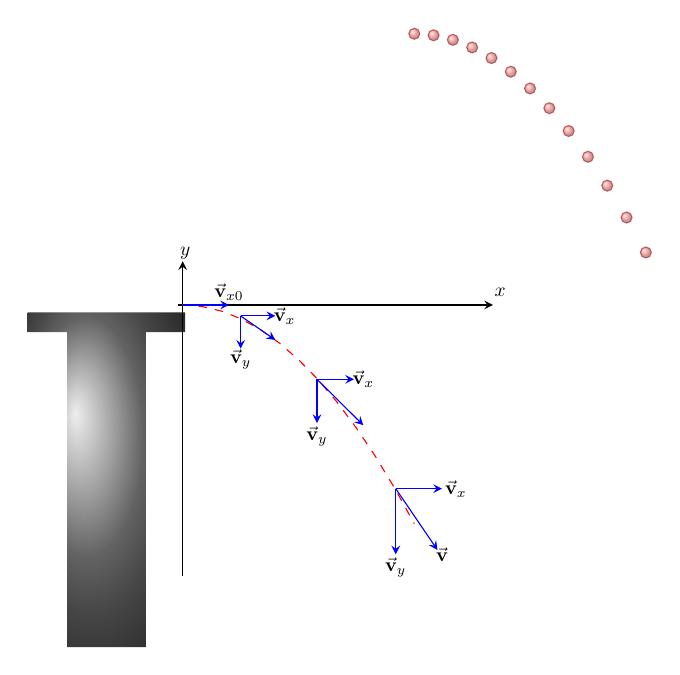
\begin{tikzpicture}
		%\draw[step=.5cm,gray,very thin] (0,0) grid (7cm,5cm);
		\shade[ball color=gray!90!white] (1,0)--(2,0)--(2,4)--(2.5,4)--(2.5,4.25)--(0.5,4.25)--(0.5,4)--(1,4)--cycle;
				\node[scale=0.7] at (2.5,5){$y$};
				\node[scale=0.7] at (6.5,4.5){$x$};
	   \begin{axis}[scale only axis,
	   	anchor=center,
	   	at={(4.41cm,2.9cm)},
	    width=4cm,
	    height=4cm,
	   	xmin=-0.1,xmax=6.7,
	   	ymin=-6.2,ymax=1,
	   	axis lines=middle,
	   	xtick=\empty,
	   	ytick=\empty,
	   	]	
	   	 \addplot+[only marks,mark=*)] {-0.2*x^2};
	   	 \addplot+[no marks,dashed] {-0.2*x^2};
	   	 
	   	
	   	 
	   	\draw[-{stealth},blue] (axis cs:1.25,-0.25)--(axis cs:1.25,-1);
	   	\draw[-{stealth},blue] (axis cs:1.25,-0.25)--(axis cs:2,-0.25);
	    \draw[-{stealth},blue] (axis cs:1.25,-0.25)--(axis cs:2.,-0.8);
	   	\node[scale=0.7] at (axis cs:2.2,-0.25){$\vec{\mathrm{\bf v}}_{x}$};
	   	\node[scale=0.7] at (axis cs:1.25,-1.25){$\vec{\mathrm{\bf v}}_{y}$};
	   	
	   	\draw[-{stealth},blue] (axis cs:2.9,-1.7)--(axis cs:2.9,-2.7);
	   	\draw[-{stealth},blue] (axis cs:2.9,-1.7)--(axis cs:3.7,-1.7);
	   	\draw[-{stealth},blue] (axis cs:2.9,-1.7)--(axis cs:3.9,-2.75);
		\node[scale=0.7] at (axis cs:3.9,-1.7){$\vec{\mathrm{\bf v}}_{x}$};
		\node[scale=0.7] at (axis cs:2.9,-3){$\vec{\mathrm{\bf v}}_{y}$};

		\draw[-{stealth},blue] (axis cs:4.6,-4.2)--(axis cs:4.6,-5.7);
		\draw[-{stealth},blue] (axis cs:4.6,-4.2)--(axis cs:5.6,-4.2);
		\draw[-{stealth},blue] (axis cs:4.6,-4.2)--(axis cs:5.5,-5.6);
		\node[scale=0.7] at (axis cs:5.9,-4.2){$\vec{\mathrm{\bf v}}_{x}$};
		\node[scale=0.7] at (axis cs:4.6,-6){$\vec{\mathrm{\bf v}}_{y}$};
		\node[scale=0.7] at (axis cs:5.6,-5.7){$\vec{\mathrm{\bf v}}$};
		
		\draw[-{stealth},blue] (axis cs:0,0)--(axis cs:1,0); 
		\node[scale=0.7] at (axis cs:1,0.3){$\vec{\mathrm{\bf v}}_{x0}$};
	
	   	\end{axis}
	   
	\end{tikzpicture}
\end{document}


